\section{Architecture générale}
Le but du projet est de permettre d'échanger et de synchroniser des documents entre différents services de stockage.\\

Pour cela, plusieurs composants sont nécessaires :
\begin{itemize}
\renewcommand{\labelitemi}{$\bullet$}
   \item Le serveur : Le serveur reçoit des instructions par notre API interne, et achemine les événements et les données d'un service à l'autre.
   \item Le client : Le client est l'interface utilisateur d'Onitu. Il échange avec le serveur via l'API interne.
   \item Les \textit{drivers} : Les \textit{drivers} sont des petits programmes à l'interface entre le serveur et les différents services de stockage comme Dropbox ou Amazon S3.
\end{itemize}

\begin{figure}
    \center
    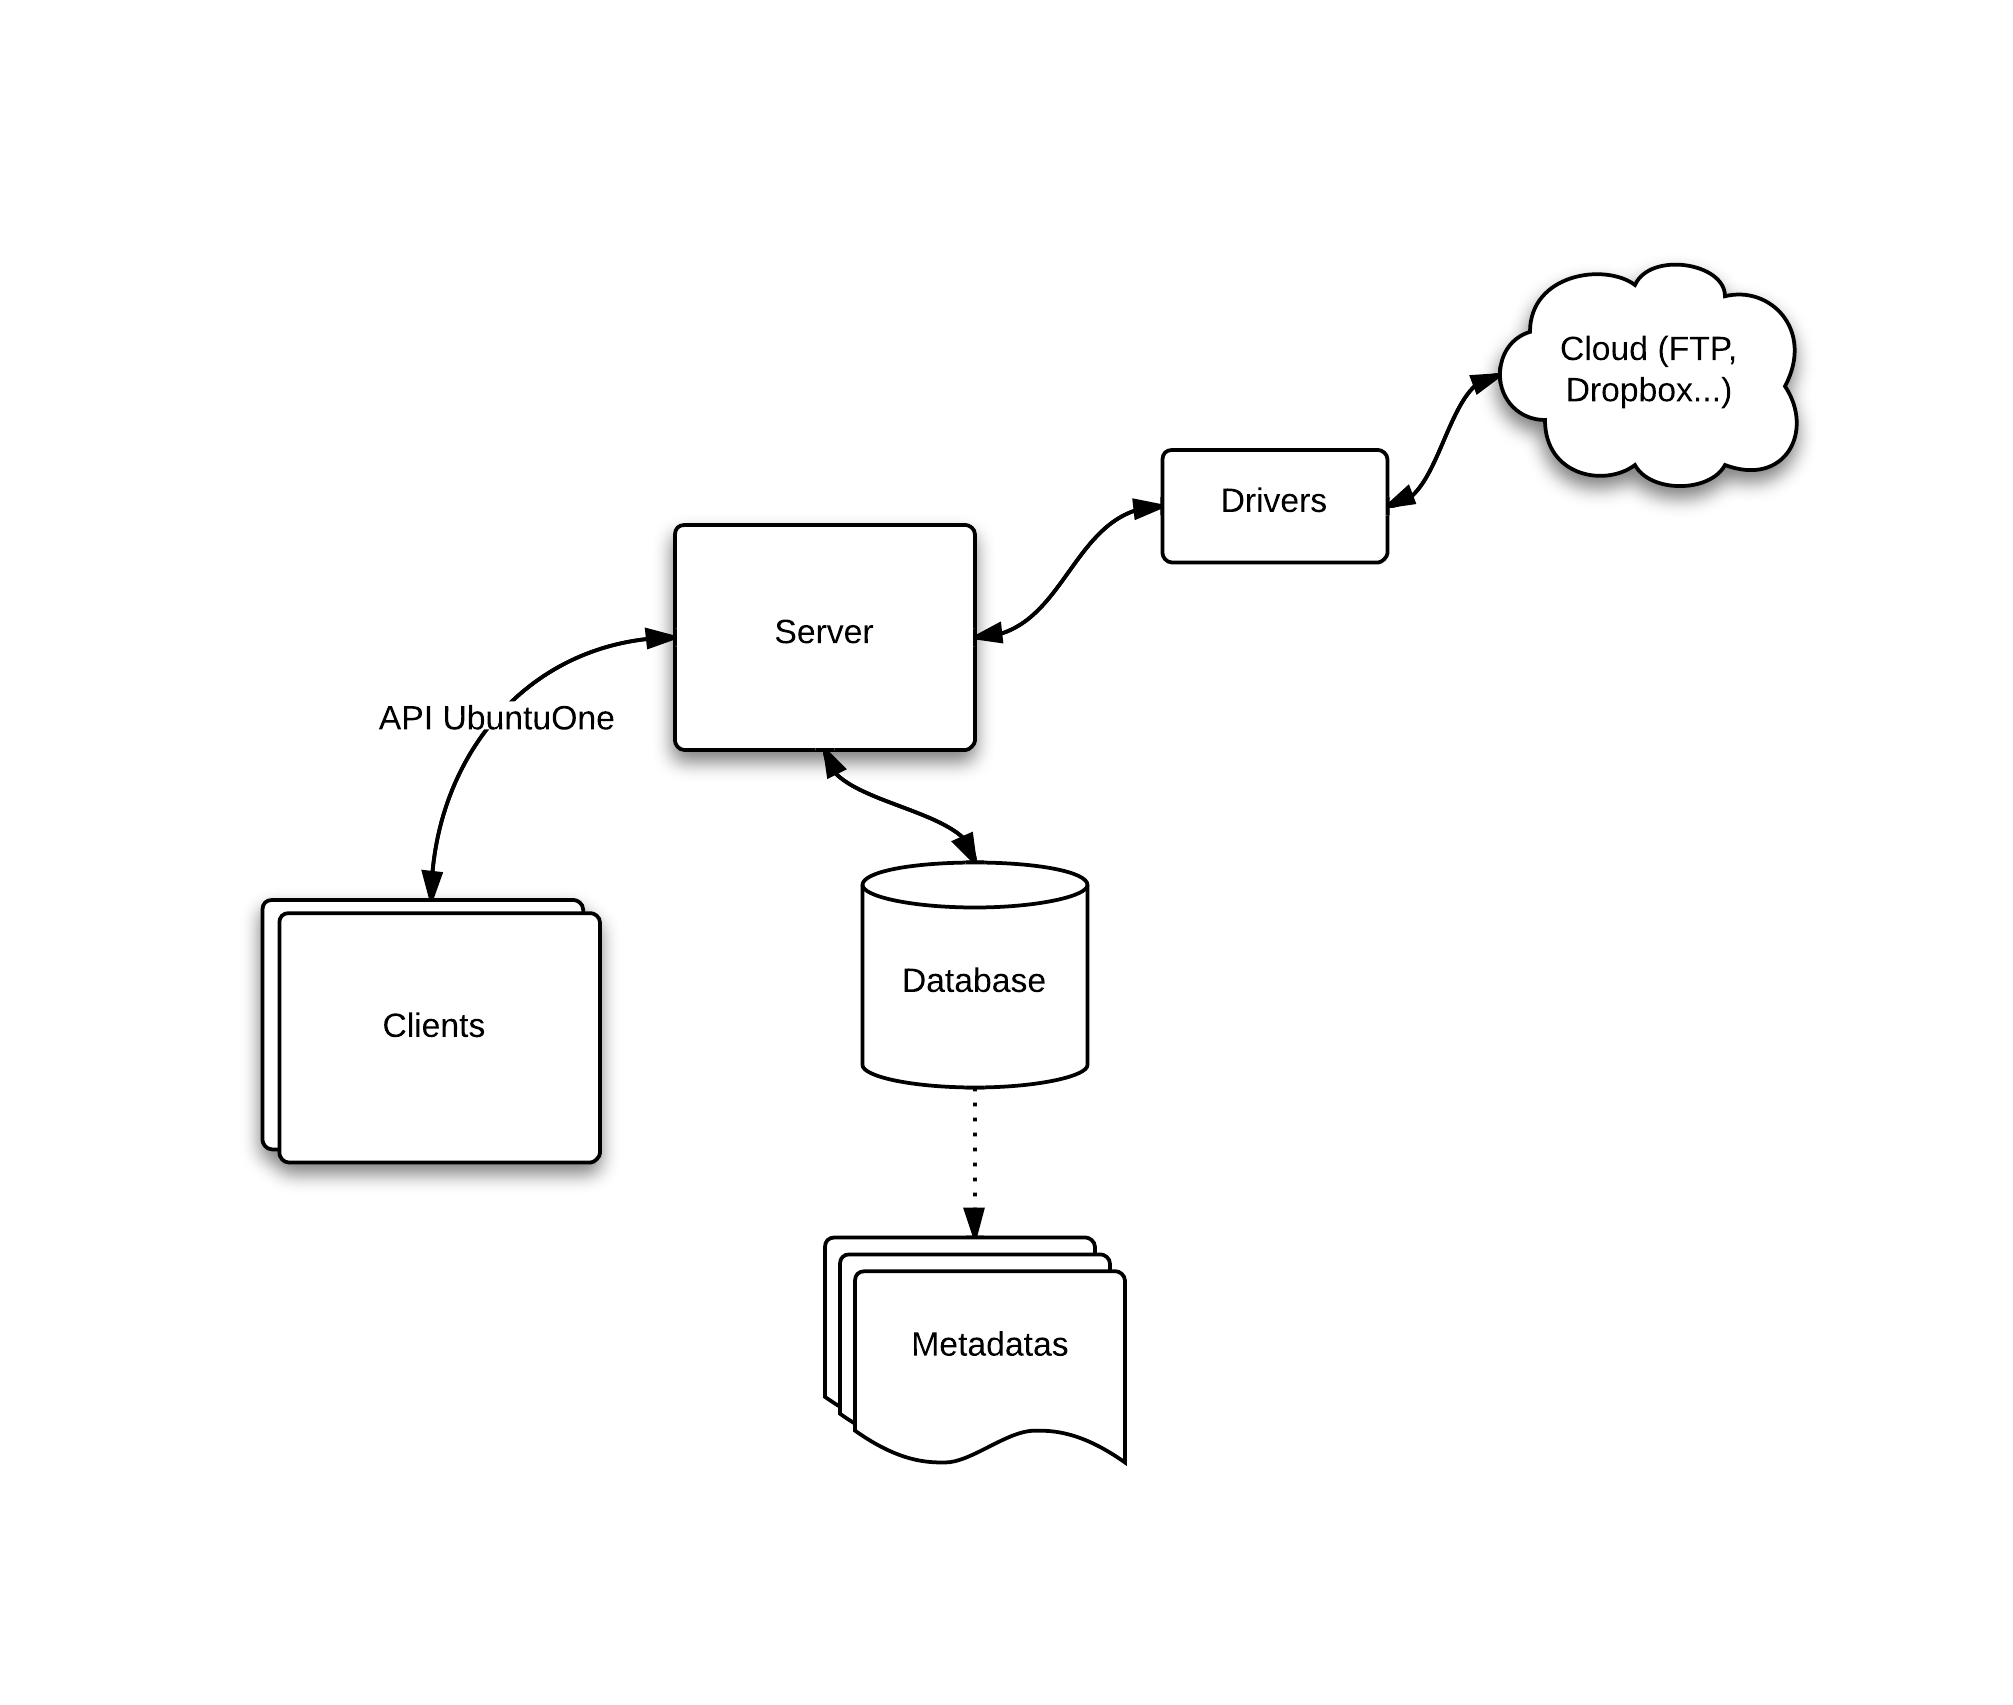
\includegraphics[scale=0.25]{architecture.png}
    \caption{Architecture générale du projet}
\end{figure}

\section{Serveur}
Le serveur est la partie centrale du projet. Il doit interpréter les instructions envoyées par les clients, et y répondre, tout en communiquant avec les drivers pour interagir avec les services de stockage utilisés par Onitu.\\

Onitu permet aux utilisateurs de choisir plusieurs moyens pour stocker leurs données. Du point de vue du serveur, cela se fait grâce aux méta-données stockées en base de données, qui contiennent les informations nécessaires aux \textit{drivers} pour récupérer les informations.\\

\section{Drivers}
Les \textit{drivers} permettent la communication entre le serveur et les différents services de stockage. Ils sont construits autour d'une interface commune, qu'ils étendent afin d'interagir avec le service auquel ils sont connectés.\\

Tous les \textit{drivers} doivent permettre d'effectuer les quatre opérations de base : la création d'un fichier, sa récupération, son édition et sa suppression (connu sous l'acronyme \textit{CRUD}, pour \textit{Create, Read, Update, Delete}).\\

Du fait du côté ouvert d'Onitu, n'importe qui peut créer son propre \textit{driver}. Ceci dit, plusieurs sont prévus et seront maintenus dans le cadre de l'EIP :
\begin{itemize}
\renewcommand{\labelitemi}{$\bullet$}
    \item \textbf{Stockage local} : Pour permettre de stocker des fichiers sur le serveur où est installé Onitu.
    \item \textbf{Dropbox/Google Drive/Amazon S3/Flickr/Evernote} : Onitu peut utiliser ces services tiers pour récupérer et stocker les fichiers, si l'utilisateur y possède un compte.
    \item \textbf{(S)FTP/WebDAV} : Des drivers permettent d'utiliser n'importe quel serveur supportant au moins un de ces protocoles. Cela permet à un utilisateur d'étendre simplement son espace de stockage sans être dépendant d'un service qu'il ne maîtrise pas.
\end{itemize}

\section{Base de données}
Les meta-données liées aux fichiers seront stockées dans une base de données, au sein du serveur.\\

Onitu étend ces méta-données en ajoutant les informations nécessaires aux \textit{drivers}. La forme de ces informations est, dans l'ensemble, laissée libre à chaque \textit{driver}.\\

Cette flexibilité est rendue possible grâce à l'utilisation d'une base de type NoSQL orientée document, LevelDB.

\section{Clients}

Le but d'Onitu n'est pas de fournir des clients, mais un serveur.

Cependant, à des fins de confort d'utilisation, une interface graphique est aujourd'hui nécessaire. C'est pourquoi nous prévoyons deux interfaces pour permettre à l'utilisateur d'interagir avec Onitu de manière plus conviviale que par la ligne de commande:
\begin{itemize}
\renewcommand{\labelitemi}{$\bullet$}
	\item Une interface Web, consultable dans tout navigateur
	\item une application graphique indépendante, écrite en Qt
\end{itemize}

Un client doit pouvoir être identifié de manière unique auprès du serveur.

\subsection{Fonctionnalités}

L'interface utilisateur est destinée à l'administrateur d'Onitu qui peut y effectuer la plupart des actions de configuration.\\

L'interface dispose ainsi de plusieurs fonctionnalités :
\begin{itemize}
\renewcommand{\labelitemi}{$\bullet$}
    \item Charger de nouveaux fichiers
    \item Éditer les dossiers et les noms de fichiers
    \item Télécharger des fichiers
    \item Ajouter, supprimer ou modifier les services externes utilisés, qui communiquent par le biais des drivers
    \item Éditer les différentes options de configuration du serveur
    \item Partager un fichier publiquement à partir d'une url unique
\end{itemize}

\section{Referee}

Le Referee (ou "\emph{arbitre}") est un composant important de l'application, car c'est par lui que transitent toutes les données en provenance, et à destination, des \emph{drivers}.

Une partie importante de la configuration du serveur concerne les règles de synchronisation du referee. En effet, ce sont ces règles qui permettent de spécifier au referee quels sont les drivers devant interagir ensemble, à quelle occasion, et avec quels fichiers interagir, sur la base d'attributs définis. C'est donc le composant qui permet de rendre Onitu extrêmement flexible sur l'utilisation que l'utilisateur souhaite en faire.

Les règles de configuration doivent aussi être personnalisables pour chaque
client. Cela doit permettre d'avoir des utilisateurs différents avec des
autorisations d'accès aux documents différentes.


\section{API publique}

Onitu doit mettre à disposition une API publique REST pour permettre de récupérer des
informations sans passer par l'interface web ou le client.

Cette API permettra notamment :
\begin{itemize}
\renewcommand{\labelitemi}{$\bullet$}
	\item de vérifier l'état d'Onitu
	\item d'intéragir avec les fichiers stockés sur Onitu
  \item De modifier les règles de configuration
\end{itemize}
